% GraspGrade paper
% Build: pdflatex main.tex  (twice, for references)
% Only standard LaTeX packages are used, so it also builds on Overleaf as is.
\documentclass[10pt,twocolumn,letterpaper]{article}

\usepackage[margin=0.85in]{geometry}
\usepackage{mathptmx}
\usepackage[scaled=0.9]{helvet}
\usepackage{courier}
\usepackage[T1]{fontenc}
\usepackage[utf8]{inputenc}
\usepackage{graphicx}
\usepackage{booktabs}
\usepackage{amsmath}
\usepackage{amssymb}
\usepackage[font=small,labelfont=bf]{caption}
\usepackage{url}
\usepackage[hidelinks]{hyperref}

\graphicspath{{figures/}}

\setlength{\tabcolsep}{4pt}
\renewcommand{\arraystretch}{1.1}

\title{\textbf{GraspGrade: Scoring First-Person Video Clips for Robot Hand
Imitation, Checked Against Touch Gloves and Motion Capture}}

% TODO: replace with the final author list and affiliation.
\author{GraspGrade Team\\
\small Hackathon submission, Push the Frontier (robotics)\\
\small Project page: \url{https://graspgrade.vercel.app}}
\date{November 3, 2026}

\begin{document}
\maketitle

\begin{abstract}
Robot hand teams want first-person human video because it is cheap and
plentiful, but most of it cannot teach a robot hand. Today clips are picked
by looking at the video only, and there is no way to check the choice against
real contact or a real robot. GraspGrade cuts first-person video into clips at
the moment of contact and gives each clip a score from 0 to 100 for how likely
it is that a robot hand can copy the grasp. Video is the only input. We build
ground truth for both steps from sensors, a touch-sensing glove for contact
timing and motion capture of hands and objects for robot copyability, and use
it to correct and score methods built from Meta SAM 3.1 and Muse Spark. The
main finding is that models which only see video pick contact timing and
copyable grasps more accurately once they are corrected with sensor ground
truth. On 22 held-out glove episodes, a vision language model asked
directly about touch, plus one timing shift learned from the glove on tuning
episodes, gives the best contact timing of the arms we compare (boundary F1
0.195 at $\pm 5$ frames, 0.376 at $\pm 15$ frames, contact IoU 0.850). On
1,426 held-out motion capture clips, the same model asked the plain question
``can a robot hand copy this?'' is at chance (AUC 0.501), while a fixed
checklist of object and hand questions reaches 0.624. The gain comes from the
checklist ($+0.117$), not from learning weights on labels ($+0.005$). The name
of the object alone reaches 0.771 when the object was labeled before, and our
score keeps 0.571 on objects it has never seen, where the object name has
nothing to say. The score is for rigid objects: a step meant to hold soft
objects back misses its pre-registered rule. Both ground truths are released
as label files with
standalone scorers, so other filters can be scored against the same sensors.
Every comparison, threshold and pass rule was written down before the held-out
data was scored.
\end{abstract}

\section{Introduction}

A robot hand that learns from human video needs clips where the hand is
visible, the touch is clear, and the grasp is one the robot hand can actually
reproduce. Most internet video fails this. In a recent study only 83 of 2,000
clips, about 4 percent, passed a quality filter \cite{doasido}. Teams usually
describe the reasons they drop a clip, but they rarely publish a score that
another team can reuse, and almost never one that is checked against a sensor
rather than against human opinion.

Two questions have to be answered before any clip is useful.

\begin{enumerate}
\item \textbf{When does a touch start and end?} The clip has to be cut at the
right frames. From video alone this is hard, because pressure is not visible.
\item \textbf{Can a robot hand copy this grasp?} A human hand reaches places a
four-finger robot hand cannot, and a robot finger is thicker than a human
finger.
\end{enumerate}

The common option today is to show a vision language model a clip and ask it
whether a robot hand can copy the grasp. On our tuning data this is close to
chance.

GraspGrade answers both questions from video alone and checks each answer
against a sensor, not against our own judgement.

\paragraph{Contributions.}
\begin{itemize}
\item A contact cutting comparison on a touch-sensing glove dataset, with
three arms built from Meta SAM 3.1 and Muse Spark, and a timing shift learned
from the glove. We report the full table, including the rows our own pipeline
loses (Section \ref{sec:num1}).
\item A copyable label for grasp clips, built from motion capture hands and
objects and a position retargeting of the human hand onto an Allegro robot
hand, with mesh collision and contact reach conditions. The label passes an
acceptance rule fixed before it was computed, and we report it at three
collision depth limits (Section \ref{sec:label}).
\item A video-only score from twelve graded checks, and six comparisons that
separate what the checklist adds from what learning adds, and what the object
name alone already tells. The score is tested on objects it has never seen
(Section \ref{sec:num2}).
\item A scope stated from data: the score is for rigid objects, and a soft
object step that was meant to widen it fails its pre-registered pass rule
(Section \ref{sec:soft}).
\item The method as one pipeline that runs on new video without sensors, using
the shift and the weights learned here (Section \ref{sec:pipeline}).
\item A benchmark release of both ground truths as label files with standalone
scorers that reproduce our numbers exactly, so any video selection rule can be
scored against the same sensors (Section \ref{sec:bench}).
\end{itemize}

Everything was run under a pre-registration discipline. Every threshold,
prompt and weight was chosen on a tuning split, and every reported number
comes from a held-out split that was scored once.

\section{Related work}

Recent work on dexterous manipulation from human video filters clips before
retargeting them. ``Do as I Do'' reports that 83 of 2,000 everyday human video
clips survive its quality check \cite{doasido}. SPIDER \cite{spider} and
ManipTrans \cite{maniptrans} retarget human hand motion to robot hands with
physics in the loop, which is accurate and expensive per clip. GraspGrade runs
before that step. It is a cheap geometric filter that decides which clips are
worth the expensive treatment, and it is scored against sensors.

For the models and data we use Meta SAM 3.1 for hand and object tracking, Meta
Muse Spark as the vision language model, HOT3D \cite{hot3d} for hand and object
motion capture, OpenGraph Ego-Tactile \cite{egotactile} for tactile gloves, and
dex-retargeting \cite{dexretargeting} for the human to robot hand mapping.

\section{Data and splits}

\paragraph{OpenGraph Ego-Tactile.} 72 episodes of first-person video at 30 fps,
138,629 frames, 1.28 hours. Both hands wear a glove with 80 taxels. The camera
is an iPhone ultrawide, about 107 degrees horizontal field of view. Splits:
50 tuning episodes, 22 held-out episodes.

\paragraph{HOT3D (Project Aria).} 136 Aria sequences from 9 persons have hand
and object pose ground truth, 480,375 RGB frames at 30 fps, fisheye,
1408 by 1408. There are 33 objects with 3D models. Splits by person: 6 persons
and 85 sequences for tuning, 3 persons and 51 sequences held out.

Both splits were drawn once with a fixed seed and never re-rolled. Neither
dataset is redistributed here.

\paragraph{Clips.} A grasp clip is cut from motion capture: two fingertips
within 15 mm of an object, one second added before and after, the object moved
at least 3 cm, and the clip passes the dataset quality check. One clip belongs
to one hand. This gives 2,385 tuning clips and 1,426 held-out clips.

\paragraph{Ground truth for contact timing.} A hand is in contact when the sum
of its 80 taxels is above 800. Pressure dropouts of 0.1 s or less are joined
and pressure blips shorter than 0.1 s are dropped, because that flicker is
threshold noise no video method can see. The raw glove and the dataset contact
labels are reported next to it as checks. The three agree on about 97 to 99
percent of frames.

\section{Definitions and thresholds}
\label{sec:defs}

Every rule below was fixed on the tuning split before the held-out split was
scored. The experiment id after each value says where it was fixed.

\paragraph{Task 1 ground truth, the cleaned glove.}
\begin{equation}
c_t = \mathbf{1}\Big[ \textstyle\sum_{i=1}^{80} p_{i,t} > 800 \Big]
\end{equation}
where $p_{i,t}$ is the pressure of taxel $i$ of one hand at frame $t$, at
30 fps. Contacts broken for 3 frames (0.1 s) or less are joined, and pieces
shorter than 0.1 s are dropped (EXP-04, EXP-14).

\paragraph{Task 1, arm B, the SAM mask rule at 10 fps.}
\begin{align}
\mathit{near}_t &= \mathbf{1}[\, d_t \le \tau_d \,]\\
m_t &= \max\big(\lVert \Delta o_{t-3 \to t} \rVert,\
      \lVert \Delta o_{t \to t+3} \rVert\big) / \sqrt{A_o}\\
\kappa_t &= \frac{\lVert \Delta o - \Delta h \rVert}
                 {\lVert \Delta o \rVert + \lVert \Delta h \rVert + 5}\\
\mathit{move}_t &= \mathit{near}_t \wedge \mathit{hand}_t \wedge
      (m_t \ge \tau_m) \wedge (\kappa_t \le \tau_\kappa)
\end{align}
Here $d_t$ is the pixel distance between the SAM hand mask and the nearest
object mask, $\Delta o$ and $\Delta h$ are the motions of the object and hand
mask centres with camera motion removed, camera motion is the median motion of
the other objects in the same window, and $A_o$ is the median object mask area.
So $m_t$ is object motion in units of object size, and $\kappa_t$ is near zero
when hand and object move together. A contact segment is a run of
$\mathit{near}_t$ that holds at least one $\mathit{move}_t$ frame. Gaps of $f$
frames or less are joined and segments shorter than 0.2 s are dropped. A
segment is also cut when the nearest object changes and stays changed for $q$
frames (EXP-22, EXP-24).

The thresholds come from a grid search on the tuning episodes,
$\arg\max [\mathrm{F1}_{\pm 15} + \mathrm{IoU}]$ over
$\tau_d \in \{2,4,8,12\}$ px, $\tau_m \in \{0.05,0.1,0.2\}$,
$\tau_\kappa \in \{0.5,0.7\}$, $f \in \{0,1,2\}$ and $q \in \{1,3,5\}$. The
50 tuning episodes chose $\tau_d = 2$ px, $\tau_m = 0.05$,
$\tau_\kappa = 0.7$, $f = 0$, $q = 3$, with shifts $\delta_s = +4$ and
$\delta_e = -1$ frames (EXP-32).

\paragraph{Task 1 timing shift, the same form for every arm.}
\begin{equation}
\delta_s = -\operatorname{med}_j(\hat{s}_j - s_j), \qquad
\delta_e = -\operatorname{med}_j(\hat{e}_j - e_j)
\end{equation}
$\hat{s}$ and $\hat{e}$ are the predicted start and end, $s$ and $e$ the glove
start and end, matched one to one within 15 frames on tuning episodes only.
Arm A gets $\delta_s = +7$ and $\delta_e = -7$ frames (EXP-29). Arm C learns
only from the tuning boundaries that Muse Spark moved, and gets $+6$ and $-4$
(EXP-36).

\paragraph{Task 1 metrics.} Predicted and glove boundaries are matched one to
one within $|\hat{s} - s| \le k$, each only to its own kind, with
$k = 5$ and $k = 15$ frames (0.167 s and 0.5 s). Then
$P$ is matches over predicted boundaries, $R$ is matches over glove
boundaries, $\mathrm{F1}_{\pm k} = 2PR/(P+R)$, and the contact IoU is the
overlap of predicted and glove contact frames over their union.

\paragraph{Task 2 ground truth, the copyable version 2 label.}
\begin{equation}
y = \mathbf{1}\big[\, \exists\, u \in U:\
\mathrm{grip}(u) \wedge \mathrm{reach}(u) \wedge \neg\,\mathrm{collide}(u) \,\big]
\end{equation}
$U$ is a shift of the whole robot hand on a 1 cm grid up to 2 cm. The three
conditions are given in Section \ref{sec:label}, and all thresholds were fixed
before computing (EXP-16).

\paragraph{Task 2 grades.}
\begin{equation}
g(x) =
\begin{cases}
1 & x \ge q_{2/3}\\
0.5 & q_{1/3} \le x < q_{2/3}\\
0 & x < q_{1/3}
\end{cases}
\end{equation}
with $q$ the terciles of the tuning clips. The raw values $x$ are listed in
Section \ref{sec:num2}.

\paragraph{Task 2 score and the rows it is compared with.}
\begin{align}
S &= 100\,\sigma\Big(w_0 + \textstyle\sum_{i=1}^{12} w_i g_i\Big)\\
R_2 &= \textstyle\frac{1}{7}\sum_{i \in \mathrm{Muse}} g_i \\
R_3 &= \sigma\Big(w_0 + \textstyle\sum_{i \in \mathrm{Muse}} w_i g_i\Big)
\end{align}
with $\sigma(z) = 1/(1 + e^{-z})$. $R_1$ is the copyable probability that Muse
Spark gives when it is asked the question directly, and $r(o)$ is the copyable
share of object $o$ on the tuning clips. The weights $w$ come from an L2
logistic regression ($C = 0.5$) on the 400 tuning clips. AUC is
$P(S^+ > S^-) + \tfrac{1}{2}P(S^+ = S^-)$, with a 95 percent interval from a
bootstrap over held-out sequences. For the unseen object rows, the hand shape
model, the terciles and the weights are all refit without the object being
scored, so $r(o)$ gives every clip the same value and sits at AUC 0.5.

\section{Task 1: when does a touch start and end?}
\label{sec:num1}

\subsection{Three arms}

All three arms take video only and output contact segments per hand at 30 fps.

\begin{description}
\item[A. Muse Spark alone.] The model sees frames at 5 fps, several frames per
call with their times, and says per frame and per hand whether the hand
touches an object. No SAM.
\item[B. SAM rule.] SAM 3.1 tracks masks for the prompts \texttt{hand} and
\texttt{small object} at 10 fps. Contact comes from mask distance plus
co-movement, that is, the object moving with the hand after camera motion is
removed (Section \ref{sec:defs}). The thresholds were chosen on the 50 tuning
episodes by leaving one episode out, and 46 of 50 folds picked the same rule.
\item[C. SAM rule plus a Muse Spark boundary check.] For every start and end
that arm B produces, Muse Spark sees about 7 frames around it at 30 fps and
picks the first or last touch frame, with a reason and a confidence.
\end{description}

Two reference rows make the numbers readable: ``always in contact'' and
``never in contact''.

\subsection{Timing shift from the glove}

Video shows a touch before the glove feels pressure, by about 0.2 s. Judged
against the glove with no correction, every video arm looks late at the start
and early at the end. Each Muse Spark arm therefore gets one constant shift per
boundary kind, learned on tuning episodes only (Section \ref{sec:defs}). Arm A
gets $+7$ frames at the start and $-7$ at the end. Arm C gets $+6$ and $-4$,
measured only on the boundaries that Muse Spark moved. The shift is two numbers
per arm. It is a calibration from sensor truth and not a new model, and the
unshifted row is reported next to it.

\subsection{Metrics}

Boundary F1 at $\pm 5$ frames and at $\pm 15$ frames, and contact IoU over all
frames (Section \ref{sec:defs}), reported pooled and per hand. The test for
the shift is a paired bootstrap over the 22 held-out episodes, 1,000 draws,
F1 at $\pm 5$ frames. The shift counts as useful only if the 95 percent
interval of the difference lies above zero.

\subsection{Results}

\begin{table}[t]
\centering
\caption{Task 1 on the 22 held-out episodes, 44 episode-hands, 574 cleaned
glove boundaries (EXP-37). The best arm is in bold. The last column is the
number of boundaries the arm produces.}
\label{tab:num1}
\small
\begin{tabular}{lcccc}
\toprule
Row & F1 $\pm 5$ & F1 $\pm 15$ & IoU & Bounds \\
\midrule
A. Muse Spark alone      & 0.074 & 0.273 & 0.821 & 400 \\
\textbf{A + shift}       & \textbf{0.195} & \textbf{0.376} & \textbf{0.850} & 358 \\
B. SAM rule              & 0.090 & 0.214 & 0.667 & 1,790 \\
C. B + Muse Spark check  & 0.112 & 0.227 & 0.679 & 1,646 \\
C + shift                & 0.137 & 0.266 & 0.690 & 1,546 \\
Always in contact        & 0.042 & 0.042 & 0.600 & 88 \\
Never in contact         & 0 & 0 & 0 & 0 \\
\midrule
Glove (ground truth)     & & & & 574 \\
\bottomrule
\end{tabular}
\end{table}

\begin{table}[t]
\centering
\caption{Paired bootstrap over the 22 held-out episodes, F1 at $\pm 5$ frames.
The first two rows were written in the plan before the run. The rest are
descriptive, added after it (EXP-37).}
\label{tab:num1boot}
\small
\begin{tabular}{lcc}
\toprule
Difference & Value & 95\% interval \\
\midrule
(A + shift) $-$ A & $+0.121$ & 0.062 to 0.172 \\
(C + shift) $-$ C & $+0.025$ & 0.019 to 0.032 \\
\midrule
C $-$ B, $\pm 5$ & $+0.022$ & 0.004 to 0.037 \\
C $-$ B, $\pm 15$ & $+0.013$ & 0.002 to 0.023 \\
(A + shift) $-$ (C + shift), $\pm 5$ & $+0.058$ & $-0.017$ to 0.119 \\
(A + shift) $-$ (C + shift), $\pm 15$ & $+0.109$ & 0.020 to 0.221 \\
\bottomrule
\end{tabular}
\end{table}

\begin{figure*}[t]
\centering
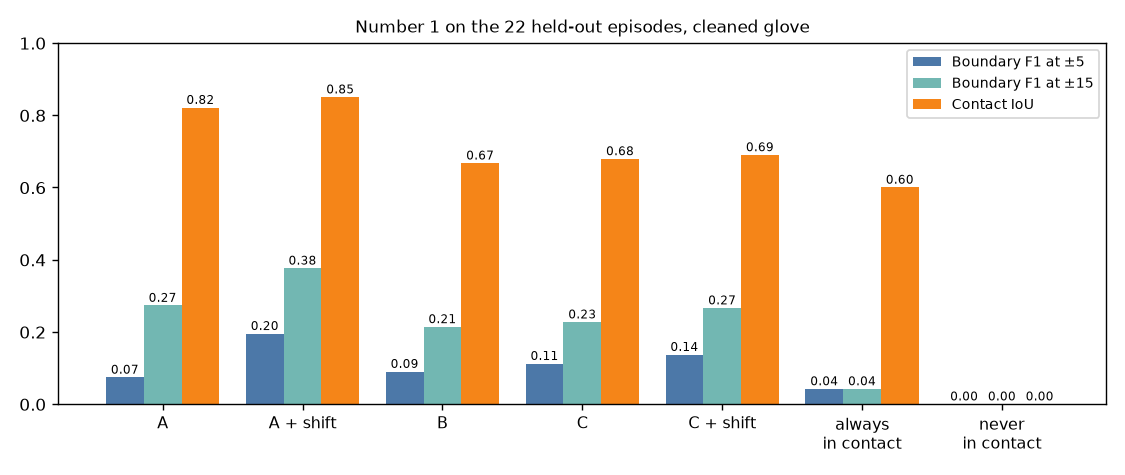
\includegraphics[width=\textwidth]{exp37_number1_final.png}
\caption{Task 1 on the 22 held-out episodes, cleaned glove ground truth
(EXP-37).}
\label{fig:num1}
\end{figure*}

Table \ref{tab:num1} and Figure \ref{fig:num1} give the result. Muse Spark
alone with the glove shift is the best row on all three metrics. The shift is
useful for both Muse Spark arms by the pre-registered test
(Table \ref{tab:num1boot}).

The Muse Spark boundary check does improve the SAM rule, by $+0.022$ at
$\pm 5$ frames, but arm C stays below arm A with the shift. The reason is
visible in the boundary counts: the SAM rule produces 1,790 boundaries where
the glove has 574, about three times too many, and arm C can only move
boundaries, never remove them. Arm B also drops from tuning to held-out, from
F1 0.153 to 0.090 at $\pm 5$ frames.

All rows are low at $\pm 5$ frames, which the plan expected. The glove measures
pressure, and pressure is not visible. At $\pm 15$ frames, half a second, arm A
with the shift finds 0.376 of the boundaries, and its contact IoU of 0.850 is
well above the 0.600 of the always in contact row.

Per hand, arm A with the shift reaches F1 0.246 at $\pm 5$ frames on the left
hand and 0.159 on the right. In 9 short episodes where arms A and B disagreed
strongly, the glove puts the left hand in contact in only 9.4 percent of
frames, and Muse Spark was right: arm A with the shift reaches IoU 0.835 there,
while arm B makes 402 boundaries for 20 real ones and reaches IoU 0.104.

\section{A copyable label from motion capture}
\label{sec:label}

Task 2 needs a ground truth for ``a robot hand can copy this grasp''. We build
it from HOT3D motion capture, with no video involved.

\subsection{First attempt and why it failed}

Our first label scaled the wrist to fingertip vectors by the ratio of robot to
human hand size, and checked collisions at link origin points only. It gave 54
percent copyable, but a check written before computing showed it mostly
measured a retargeting side effect. Robot fingertips floated about 25 mm off
cans that the person held firmly, and the copyable share per person tracked
hand length, from 29 to 74 percent. Faithful retargeting instead called 94 to
96 percent of grasps copyable, because origin-point collisions miss the thick
robot fingers. No method passed the acceptance rule, so the label was put on
hold and rebuilt.

\subsection{Copyable, version 2}

The thresholds and the acceptance rule were written down before computing.

For each clip we take the contact frame and the clip's hand. The human hand is
mapped onto an Allegro hand by position retargeting, which fits Allegro
fingertips and finger bases to the human ones with a free hand base. The
Allegro surface is about 300 sampled points on the visual mesh of each of its
21 links, placed by forward kinematics. The hand may shift up to 2 cm on a 1 cm
grid. A clip is copyable if one shift passes all three conditions:

\begin{enumerate}
\item \textbf{Grip.} The Allegro thumb tip and one more Allegro fingertip are
within 1.5 cm of the object surface.
\item \textbf{Reach.} Every human finger that touches the object, that is a tip
within 15 mm, has its Allegro fingertip within 2.0 cm of that human fingertip.
\item \textbf{No collision.} No Allegro mesh point is more than 5 mm inside the
object.
\end{enumerate}

The acceptance rule, fixed in advance, asked for a copyable share between 20
and 80 percent and a rank correlation of hand length with the label inside
objects of at most 0.1. The label passes both: 47.0 percent copyable on tuning
clips, and a hand size correlation of $+0.04$, with 44 to 54 percent by person.
On held-out clips the same fixed rule gives 46.4 percent, and the per-object
shares agree between the splits with a rank correlation of 0.85.

Failures make physical sense. Collision is the binding condition for 25.5
percent of clips, reach for 10.9 percent and grip for 3.9 percent. The thicker
Allegro fingers go into flat or crowded objects such as a keyboard or a
spatula, and the hand cannot span a wide bowl or plate the way the human did.
By object, the share runs from 1 percent for a keyboard to 96 percent for a
small holder.

\begin{figure*}[t]
\centering
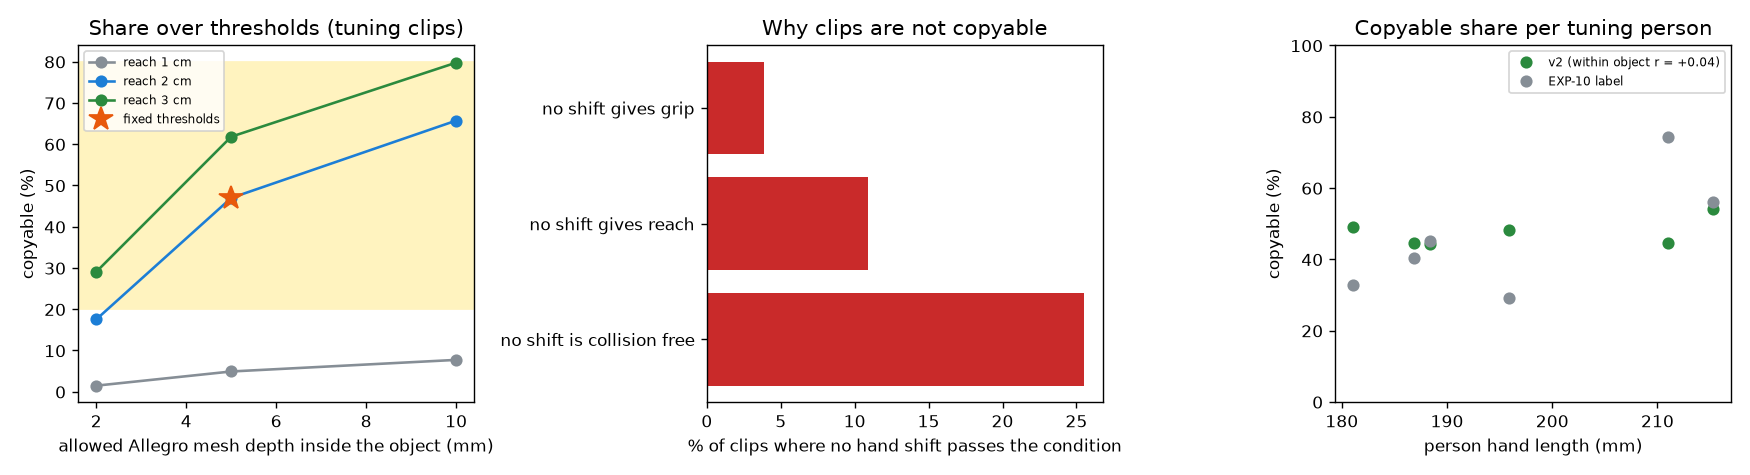
\includegraphics[width=\textwidth]{exp16_copyable_v2.png}
\caption{The copyable version 2 label. Left: the share for other reach and
depth limits, with the fixed choice starred. Middle: which condition no hand
shift can meet. Right: the share per tuning person for version 2 (green) and
for the first label (grey). EXP-16.}
\label{fig:label}
\end{figure*}

\begin{figure}[t]
\centering
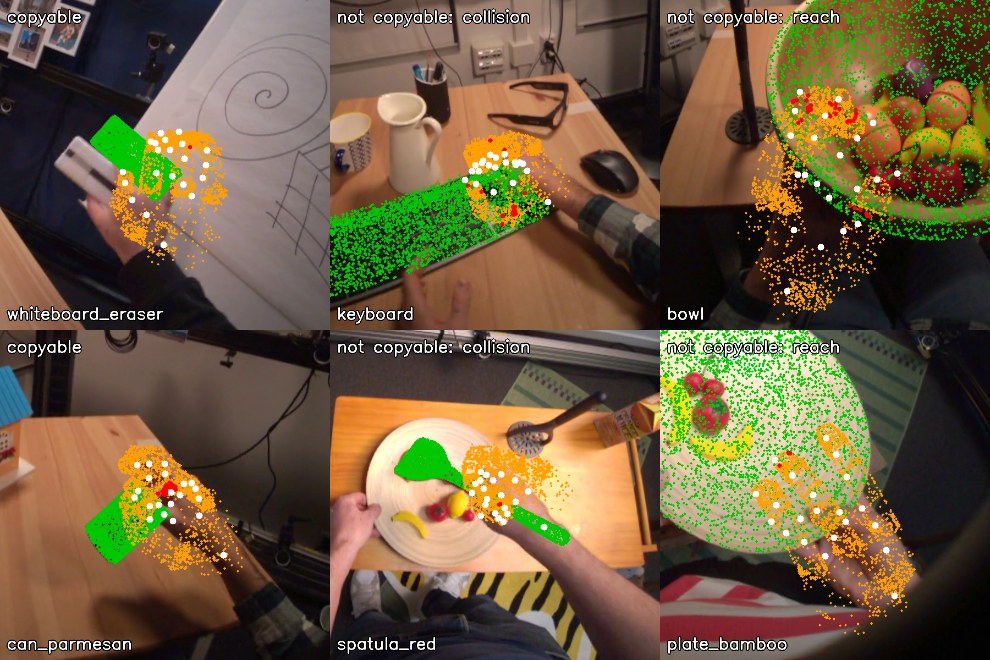
\includegraphics[width=\columnwidth]{exp16_examples.jpg}
\caption{Two tuning clips per outcome. Green is the object model, white the
human hand, orange the Allegro mesh points and red the points more than 5 mm
inside the object. Left: copyable. Middle: collision. Right: reach (EXP-16).}
\label{fig:labelex}
\end{figure}

\paragraph{The main weakness of the label.} The share depends strongly on the
collision depth limit: 18 percent at 2 mm, 47 percent at 5 mm and 66 percent at
10 mm (Figure \ref{fig:label}). The 5 mm limit is about the size of the motion
capture and model error, so the label is partly a statement about how much the
robot hand overlaps the object within measurement error. The limit was fixed
before computing, we report the whole curve, and Section \ref{sec:depth} scores
the held-out result at 2 mm and 10 mm as well.

\section{Task 2: does the score pick clips a robot hand can copy?}
\label{sec:num2}

\subsection{What decides the label: the object, not video quality}

The first checklist asked about video quality. On the version 2 label it
carries almost no signal. Leaving one tuning person out, the three video
checks reach AUC 0.529 and the hand shape seen in video 0.521. Knowing only
which object is grasped reaches 0.741, and the video checks add about 0.01 on
top of it (EXP-17). So the checklist moved from video quality to questions
about the object.

\subsection{The score}

Each clip gets twelve graded checks. Each grade is high, mid or low, coded 1,
0.5 and 0. A logistic regression on 400 tuning clips turns them into a score
from 0 to 100. We use a logistic regression and not a decision tree, so that
every weight is readable and every check contributes in a fixed direction.

\paragraph{Three local checks, no API call.} Camera stability: minus the 90th
percentile of camera motion over the clip, from corner tracking and a RANSAC
similarity fit between frames. Hand shape fit: the probability from a logistic
regression on ten MediaPipe hand features during the contact, trained on
tuning clips. Action completeness, a fixed rule and not a tercile: half the sum
of two indicators, one for the second before contact and one for the second
after it, each true when the hand is seen in at least 50 percent of frames and
the wrist moves at least 3 percent of the frame width. Checks of the checks:
camera motion against headset rotation from motion capture correlates at 0.93
(Spearman), and the MediaPipe hand label matches the motion capture hand in
96.5 percent of frames (EXP-12).

\paragraph{Two SAM 3.1 checks.} Visibility: the share of frames where SAM
found both the hand and the object. Contact clarity: the share of contact
frames with $d_t \le 3$ px, minus the same share over the reach and release
frames. Both use the masks of the prompts \texttt{hand} and
\texttt{small object} at 10 fps, and both are graded by the tuning terciles.
Visibility turned out to have only two effective grades, because about 70
percent of clips have full visibility (EXP-38).

\paragraph{Seven Muse Spark grades.} Six object items plus finger occlusion.
The object items are size next to the hand, shape, thickness, width the hand
must wrap, handle and free space around the object. High always means easier
for a large four-finger robot hand, and the anchors use the visible human hand
as the ruler, about 19 cm from wrist to middle fingertip.

The object items were settled by two free checks before any paid call. First,
whether object geometry can carry the signal that the object name carries.
Seven size and shape numbers taken from the 3D models reach AUC 0.695 when a
person is left out and 0.673 when the object itself is left out, against 0.742
and 0.500 for the object name (EXP-18, Figure \ref{fig:geom}). Second, whether
coarse three-level stand-in grades keep that signal: they reach 0.683 and
0.666 (EXP-19). Both checks had to clear a 0.65 bar set in advance, and both
did.

\begin{figure*}[t]
\centering
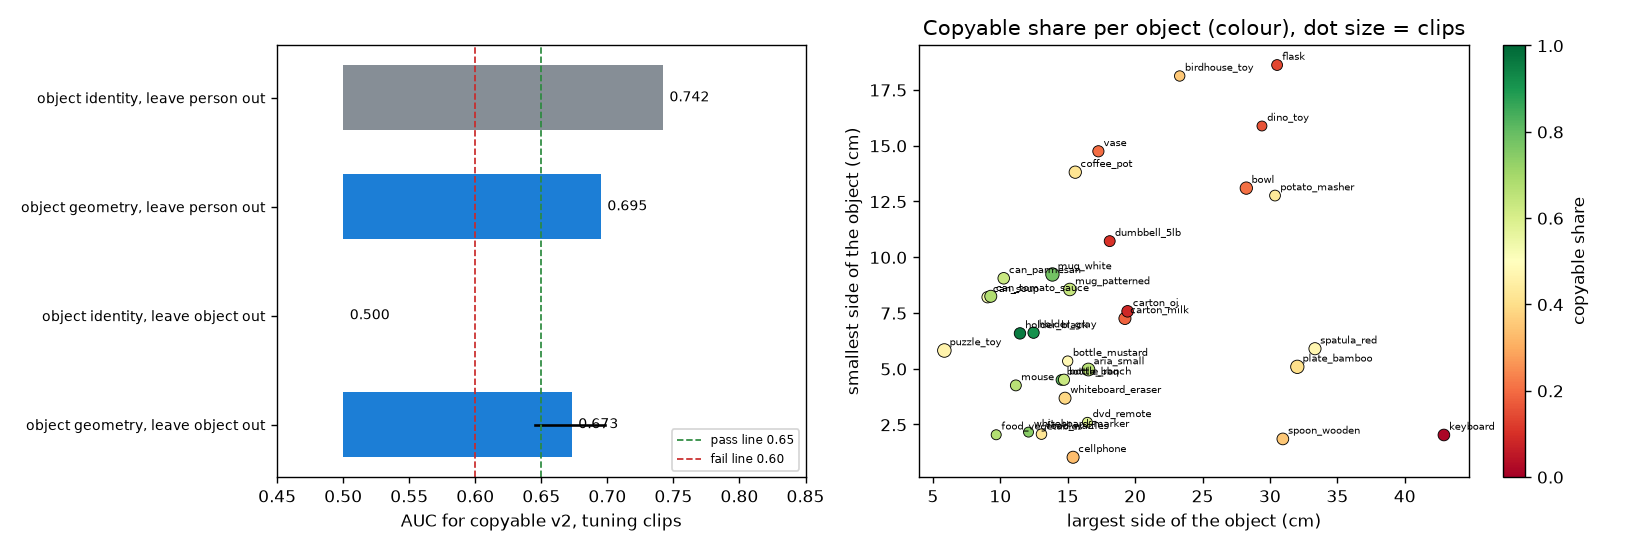
\includegraphics[width=\textwidth]{exp18_object_geometry.png}
\caption{Object geometry from the 3D models against object identity, on tuning
clips (EXP-18). Geometry still works when the object is left out of training, where
identity cannot work at all.}
\label{fig:geom}
\end{figure*}

\subsection{What is compared}

Six comparisons, all written down before the held-out run.

\begin{enumerate}
\item Our score against Muse Spark asked the same question with no checklist.
\item An object name reference: the copyable share of each object on the tuning
clips, handed to each held-out clip. It needs a label for every object, so it is
a reference and not a video method.
\item Muse Spark alone against Muse Spark plus our checks, that is GraspGrade
as a layer on an existing filter.
\item Comparisons 1 and 2 again on objects the score has never seen, with every
learned part refit without the object being scored.
\item Three rows on the same clips: Muse Spark alone, the checklist with equal
weights, and the checklist with learned weights. This separates what the
checklist adds from what learning adds.
\item Our score with the object rate added when 0, 5, 20 or all labeled tuning
clips of the object exist.
\end{enumerate}

AUC is reported with a 95 percent bootstrap interval that resamples the 51
held-out sequences, not single clips, because clips from one sequence are
related. Paired differences use the same sequences for both rows.

\subsection{Results}

\begin{table}[t]
\centering
\caption{Task 2 on the 1,426 held-out clips, 3 persons, 46.4 percent copyable.
``Top 20\%'' is the share of copyable clips in the top fifth of the ranking
(EXP-40).}
\label{tab:num2}
\small
\begin{tabular}{lccc}
\toprule
Row & AUC & 95\% interval & Top 20\% \\
\midrule
\textbf{Our score} & \textbf{0.624} & 0.589 to 0.661 & 59.4\% \\
1. Muse Spark alone & 0.501 & 0.469 to 0.529 & 46.9\% \\
2. Object name reference & 0.771 & 0.744 to 0.792 & 79.4\% \\
3. Muse alone + our checks & 0.624 & 0.590 to 0.661 & 62.6\% \\
\midrule
\multicolumn{4}{l}{\emph{Comparison 4, objects never seen in training}} \\
Our score & 0.571 & 0.534 to 0.609 & \\
Object name reference & 0.500 & by construction & \\
Muse Spark alone & 0.501 & 0.469 to 0.529 & \\
\bottomrule
\end{tabular}
\end{table}

\begin{table}[t]
\centering
\caption{Comparison 5, what the checklist adds and what learning adds. Muse
Spark grades only, paired over the 51 held-out sequences (EXP-40).}
\label{tab:num2c5}
\small
\begin{tabular}{lccc}
\toprule
Row or difference & Value & 95\% interval & Gain \\
\midrule
R1 Muse Spark alone & 0.501 & 0.469 to 0.529 & \\
R2 checklist, equal weights & 0.617 & 0.579 to 0.659 & \\
R3 checklist, learned & 0.622 & 0.588 to 0.661 & \\
\midrule
R2 $-$ R1 (the checklist) & $+0.117$ & 0.073 to 0.166 & yes \\
R3 $-$ R1 & $+0.122$ & 0.081 to 0.166 & yes \\
R3 $-$ R2 (learning) & $+0.005$ & $-0.019$ to 0.032 & no \\
Ours $-$ R3 (other checks) & $+0.001$ & $-0.011$ to 0.013 & no \\
\bottomrule
\end{tabular}
\end{table}

\begin{figure*}[t]
\centering
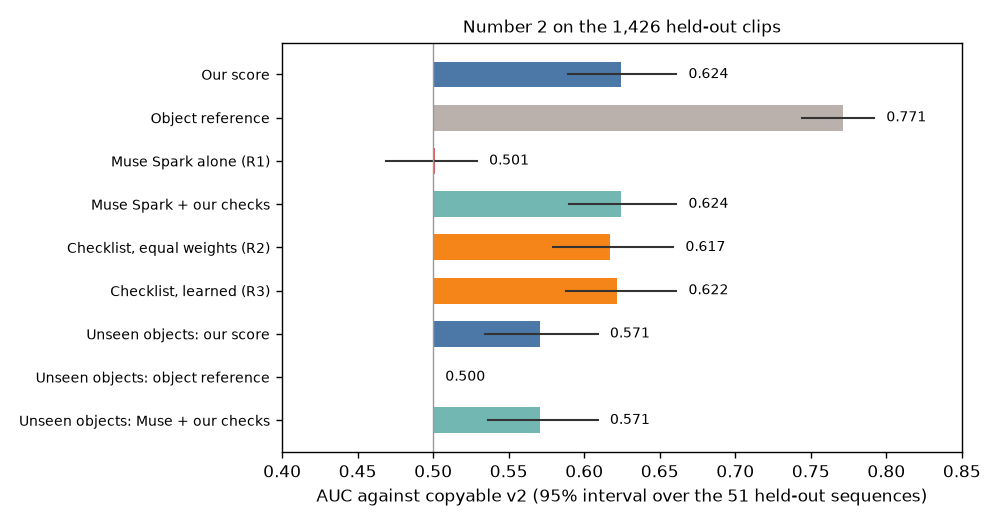
\includegraphics[width=\textwidth]{exp40_number2_final.png}
\caption{Task 2 on the 1,426 held-out clips (EXP-40).}
\label{fig:num2}
\end{figure*}

\paragraph{The checklist is what works, not learning.} Muse Spark asked the
plain question cannot tell copyable from non-copyable clips at all
(AUC 0.501, Table \ref{tab:num2}). The same grades averaged with no learning
at all reach 0.617. Learning the weights on 400 labeled clips adds $+0.005$,
and the interval does not separate that from zero. The local and SAM checks
add $+0.001$ on top (Table \ref{tab:num2c5}). So the useful part is the
question set, not the labeled training data, and the method can be used
without labels.

The score is stable across the three held-out persons, at 0.603 to 0.638, and
59.4 percent of the clips in its top fifth are copyable against a base rate of
46.4 percent. Used as a layer on top of Muse Spark alone it gives the same
0.624.

\paragraph{The object name beats our score.} The copyable share of the object,
taken from tuning labels, reaches 0.771. That is the strongest row in the
table, and our score loses to it. It is a reference and not a video method,
because the held-out persons grasp the same 33 objects as the tuning persons,
and because a new object has no share. When every learned part is refit
without the object being scored, our score keeps 0.571 and the object
reference drops to 0.500 by construction. Video of objects nobody has measured
is the case the score is built for.

\paragraph{The score ranks objects, not grasps.} Inside a single object, over
the 13,524 clip pairs that share an object, our score is at chance
(0.506, interval 0.461 to 0.544). Inside one object and one person it is
0.484. Per object, for the 27 held-out objects with at least 5 clips of each
kind, it is above 0.5 for 14 of 27, with a median of 0.502 and a range of
0.358 to 0.640. This is not for lack of spread in the label: on tuning clips
all 33 objects have both copyable and not copyable grasps, and 24 of them are
between 20 and 80 percent copyable. Comparison 6 says the same from the other
side: once 5 or more labeled clips of an object exist, the object rate alone
is as good as the combination, and adding our score to it gains nothing
($+0.004$ at 5 clips, $-0.003$ with all clips). The object rate added to our
score gains $+0.099$ to $+0.147$ in the other direction. The object rate is the
stronger of the two wherever it exists.

\paragraph{Which failures it sees.} Against clips that fail only on grip, the
score reaches 0.682. Against reach failures, 0.636. Against collision
failures, which are the most common, 0.611.

\paragraph{Learned weights.} The largest weights are object shape (1.252),
object width (0.922), finger occlusion (0.481), hand shape fit (0.434) and
object size (0.391). Camera stability and visibility end up near zero, the
first because almost no clip in HOT3D has an unstable camera, the second
because visibility has only two effective grades.

\subsection{How much the depth limit matters}
\label{sec:depth}

\begin{table}[t]
\centering
\caption{Task 2 held-out AUC at three collision depth limits. Nothing is
learned again: all weights come from the 5 mm label on the 400 tuning clips,
and only the held-out label being judged changes (EXP-41).}
\label{tab:depth}
\small
\begin{tabular}{lccc}
\toprule
Row & 2 mm & 5 mm & 10 mm \\
\midrule
Held-out copyable share & 19.9\% & 46.4\% & 64.7\% \\
\midrule
Our score & 0.521 & \textbf{0.624} & 0.632 \\
Muse Spark alone & 0.417 & 0.501 & 0.541 \\
Object name reference & 0.761 & 0.771 & 0.774 \\
Checklist, equal weights & 0.488 & 0.617 & 0.624 \\
Checklist, learned & 0.506 & 0.622 & 0.629 \\
Our score, unseen objects & 0.504 & 0.571 & 0.585 \\
Our score inside an object & 0.505 & 0.506 & 0.504 \\
\bottomrule
\end{tabular}
\end{table}

\begin{figure*}[t]
\centering
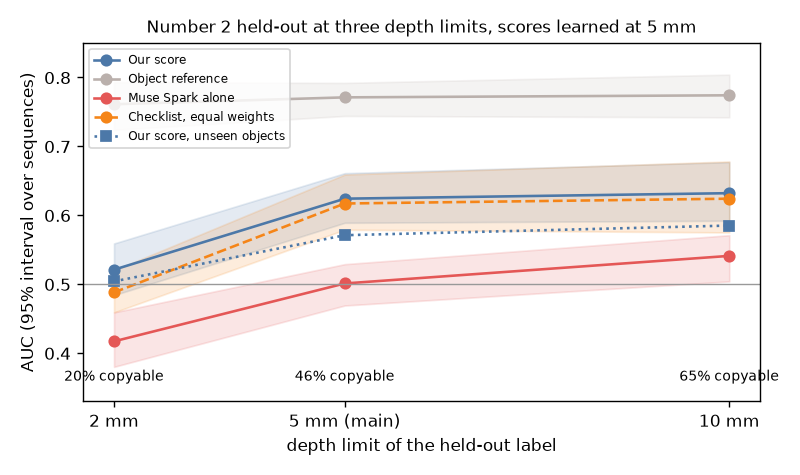
\includegraphics[width=\textwidth]{exp41_number2_depth.png}
\caption{Task 2 held-out at three collision depth limits (EXP-41).}
\label{fig:depth}
\end{figure*}

The plan said to report the held-out result at 2 mm and 10 mm as well, and to
learn nothing again. Table \ref{tab:depth} and Figure \ref{fig:depth} give it.
At 10 mm the picture holds: our score 0.632, Muse Spark alone 0.541, the
checklist adds, learning does not. At 2 mm, where only 20 percent of clips are
copyable, our score falls to chance (0.521, the interval covers 0.5) and Muse
Spark alone ranks clips the wrong way round (0.417). Our score still beats Muse
Spark alone there, but only because Muse Spark alone is below chance. The
object name reference stays at 0.76 to 0.77 at every depth.

So the task 2 result holds for the 5 mm limit that was fixed in advance and for
a looser one, and it does not hold for a stricter one. We report this as a
limit of the result, not as a choice between labels.

\section{Scope: rigid objects}
\label{sec:soft}

The score is for rigid objects. All 33 HOT3D objects in task 2 are tracked as
rigid bodies, and in the labels of two team members only 5 of them, squeeze
bottles and cartons, are squeezable and the rest are rigid. A soft object
changes shape in the hand, so its size and shape do not settle the question.

To use the score on video with soft objects, those clips have to be taken out
first. We tested one way to do this: one more Muse Spark question per clip, is
this object rigid, squeezable, soft or unsure? Soft or unsure means no score
and a note that the clip needs a touch check. The check does not meet its
rule.

\paragraph{Ground truth and rule, both fixed before any call.} Two team members
labeled all 104 object names rigid, squeezable or soft on their own, then
agreed a single label. Agreement before settling was 81.7 percent with Cohen's
kappa 0.613. The pass rule was at least 70 percent of soft segments held back
and at most 10 percent of rigid HOT3D clips held back. HOT3D tracks every
object as a rigid body, so any HOT3D clip held back counts as a mistake. There
is no verdict with fewer than 20 soft segments or 4 soft objects.

\begin{table}[t]
\centering
\caption{The soft object check against its pre-registered rule (EXP-42).}
\label{tab:soft}
\small
\begin{tabular}{lccc}
\toprule
Metric & Value & Rule & Met \\
\midrule
Soft segments held back & 51.7\% & $\ge 70\%$ & no \\
Rigid HOT3D clips held back & 2.1\% & $\le 10\%$ & yes \\
\midrule
\multicolumn{4}{l}{\textbf{Verdict: fail}} \\
\bottomrule
\end{tabular}
\end{table}

\begin{figure*}[t]
\centering
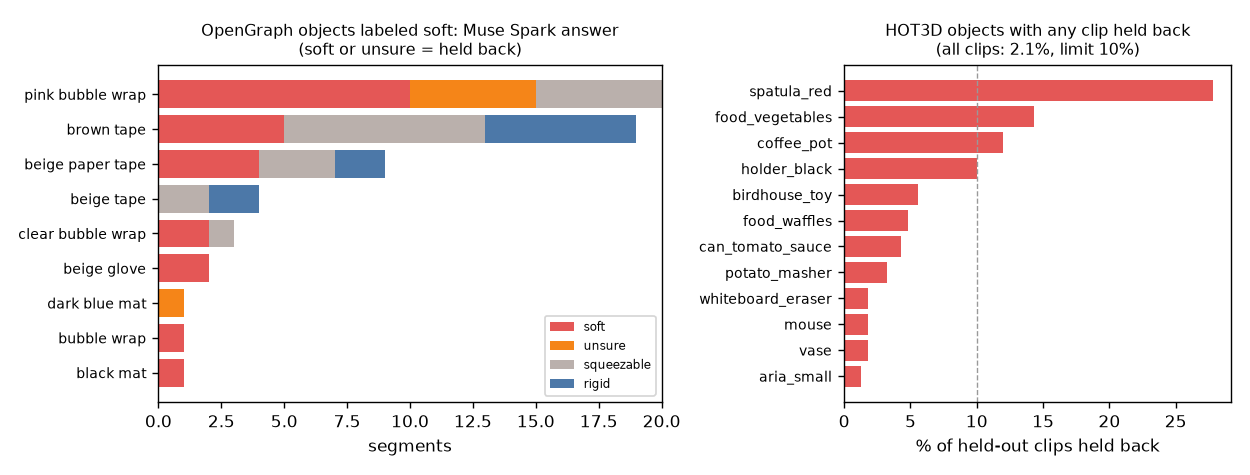
\includegraphics[width=\textwidth]{exp42_soft_check.png}
\caption{Muse Spark answers on the soft OpenGraph objects, and the HOT3D
objects it holds back (EXP-42).}
\label{fig:soft}
\end{figure*}

The check fails (Table \ref{tab:soft}). All 1,782 items returned a parsed
answer on the first pass. Muse Spark leaves rigid HOT3D clips alone, holding
back only 2.1 percent of 1,426, which satisfies the second half of the rule.
But it holds back only 31 of 60 segments labeled soft. The misses are almost
all tape: the three tape names carry 32 of the 60 soft segments and only 28
percent of those are held back, while the other six soft objects are held back
in 22 of 28 segments. Bubble wrap, gloves and mats are mostly caught. The check
also holds back 18.1 percent of rigid OpenGraph segments, which the rule did
not measure.

Two notes. Tape is a hard case for the labelers too: for two of the three tape
names the two labelers disagreed before settling, one saying squeezable and
the other soft. And dropping the held-back HOT3D clips leaves the task 2 AUC
the same, 0.624 before and 0.625 after, so the failed step does not damage the
main result. It does not do the job it was added for. A ``soft or unsure''
answer from a vision language model is not enough to keep soft objects out of
a geometric score, so the scope stays at rigid objects.

\section{The method as one pipeline}
\label{sec:pipeline}

The steps below run on first-person video with no sensors. They need the video
and calls to SAM 3.1 and Muse Spark, and they use the timing shift and the
checklist weights learned here.

\begin{enumerate}
\item Take frames at 5 fps and ask Muse Spark, for each hand, whether it
touches an object.
\item Move each contact start 7 frames (about 0.23 s) later and each end 7
frames earlier. This shift was learned from the touch gloves.
\item Cut a grasp clip for each contact, from about one second before the
touch to one second after the release, and get hand and object masks from
SAM 3.1 at 10 fps.
\item Grade the twelve checks of each clip, seven from Muse Spark, two from the
SAM masks and three computed from the video, as high, mid or low, and turn
them into a score from 0 to 100 with the learned weights.
\item Keep the clips with high scores for robot training. The viewer offers
three cut-offs: strict (70 or more), balanced (50 or more) and volume (30 or
more).
\end{enumerate}

Steps 1 and 2 are the best arm of task 1, and step 4 is the score of task 2.
The two were measured on separate datasets, because neither of our datasets
has both a touch glove and hand and object motion capture. Task 2 clips were cut from
motion capture, not by steps 1 and 2, so the joined pipeline has not been
scored end to end.

\section{The ground truth as a benchmark}
\label{sec:bench}

Training robots on human video needs a rule that picks the segments to use.
The benchmark compares the segments or scores that such a rule produces with
the sensor ground truth, and returns a score. Our heaviest and most checked
work is this ground truth, not the checklist. We release both parts, labels
only, with standalone scorers that need nothing from this project.

\begin{enumerate}
\item Make a result file. Task 1: for each episode, a list of contact segments
$[\mathit{start}, \mathit{end}]$ per hand. Task 2: one score per clip.
\item Run \texttt{score\_number1.py} on the segments file, or
\texttt{score\_number2.py} on the scores file.
\item Read the score. Task 1: boundary F1 at $\pm 5$ and $\pm 15$ frames and
contact IoU. Task 2: AUC and AUC per person.
\end{enumerate}

Reference scores: for task 1, ``always in contact'' gives F1 0.042 at
$\pm 5$ frames and IoU 0.600, and the best method here gives 0.195 and 0.850.
For task 2, the object name reference gives AUC 0.771 and our checklist score
0.624. In task 2 the same objects appear in the tuning and the held-out
clips, so the object name reference is strong. A video method should also be
checked on objects it has not seen. The files are:

\begin{itemize}
\item \texttt{number1/ground\_truth.json}: per episode and hand, contact
segments from the cleaned glove and from the raw glove, as frame ranges at
30 fps. 50 tuning episodes with 955 contacts and 22 held-out episodes with 287.
\item \texttt{number2/clips.csv}: per clip, where it is, the copyable label,
the first condition that fails, and the label at the 2 mm and 10 mm depth
limits. 2,385 tuning clips and 1,426 held-out clips over 33 objects.
\end{itemize}

The two scorers were written apart from the project code and need only numpy,
pandas and scikit-learn. They reproduce the project numbers exactly on every
case we checked, including boundary F1, contact IoU and the object share
reference AUC with its bootstrap interval. No video, sensor value or motion
capture pose is redistributed. Task 1 labels can be shared under CC BY 4.0.
Task 2 labels derive from HOT3D hand data, so they go out under
CC BY-NC-SA 4.0 and may not be sold. This is our reading of the license texts
and not legal advice.

\section{Cost}

Every paid call is cached, so a rerun sends only what is missing, and all
reported numbers can be recomputed with no API call.

\begin{table}[t]
\centering
\caption{Meta Model API spend, \$143.27 of a \$150 credit.}
\label{tab:cost}
\small
\begin{tabular}{lr}
\toprule
Step & Cost \\
\midrule
Pilots, prompt checks and tuning checks & \$19.06 \\
Task 1: SAM on 50 tuning episodes & \$11.89 \\
Task 1: SAM on 22 held-out episodes & \$5.45 \\
Task 1: arm A on held-out & \$12.44 \\
Task 1: arm C, tuning sample and held-out & \$30.28 \\
Task 2: SAM on all clip windows & \$26.48 \\
Task 2: Muse Spark checklist and baseline & \$28.56 \\
Soft object check & \$9.11 \\
\midrule
Total & \textbf{\$143.27} \\
\bottomrule
\end{tabular}
\end{table}

Two choices did most of the saving. SAM at 10 fps gives the same ids and masks
as at 30 fps, with a mask IoU of 0.97 to 0.99 on hands and the grasped object,
which cuts SAM cost to a third (EXP-05). Overlapping clips of one sequence
share one SAM window, so the task 2 SAM bill covered 1,826 clips with 513
windows for \$26.48. SAM on all 2,152 usable grasp clips as single clips would
have cost about \$59 (EXP-07, EXP-11).

\section{Limitations}

\begin{itemize}
\item The robot check is geometric, not a physics test, and it uses one robot
hand, the Allegro. It says that the hand can reach and hold the grasp without
going into the object. It does not promise that the robot succeeds.
\item The task 2 result depends on the collision depth limit. It holds at the
5 mm limit fixed in advance and at 10 mm, and not at 2 mm
(Section \ref{sec:depth}).
\item The object name alone predicts copyability better than our score when
the object has labels, and our score does not rank two grasps of the same
object (AUC 0.506 inside an object).
\item The score is for rigid objects. The soft object step does not pass its
rule, so soft objects are not yet reliably kept out of the score.
\item The two tasks were measured on separate datasets, and the joined
pipeline of Section \ref{sec:pipeline} has not been scored end to end.
\item The score has not been tested on a second dataset with new objects,
persons and cameras.
\item Contact timing is low at $\pm 5$ frames for every arm, because the glove
measures pressure and video cannot see pressure. The strong rows are at
$\pm 15$ frames and in contact IoU.
\item The HOT3D images are fisheye and stay raw. Undistorting them made
MediaPipe worse, dropping hand detection from 70.6 to 60.3 percent, so a rule
set in advance kept the raw frames.
\item MediaPipe finds gloved hands poorly on the OpenGraph videos, from 14
percent to 100 percent of frames depending on the background. Task 1 therefore
uses SAM and not MediaPipe, and task 2 runs on HOT3D, where hands are bare.
\item The held-out set for task 2 has three persons, and the clips come from
one glove setup and one motion capture setup. Everything here is lab data.
\end{itemize}

\section{Conclusion}

Models that only see video pick contact timing and copyable grasps in
first-person video more accurately once they are corrected with sensor ground
truth. Two results hold on held-out data.

\begin{table}[h]
\centering
\caption{The two headline numbers on held-out data (EXP-37, EXP-40). Muse
Spark alone is asked the question directly.}
\label{tab:headline}
\small
\begin{tabular}{lcc}
\toprule
Question & Muse Spark alone & Our method \\
\midrule
Contact timing, F1 $\pm 5$ & 0.074 & 0.195 \\
Contact timing, IoU & 0.821 & 0.850 \\
Copyable grasps, AUC & 0.501 & 0.624 \\
\bottomrule
\end{tabular}
\end{table}

For contact timing, a vision language model asked directly about touch, plus
one constant shift learned from a touch glove, beats a tracking rule built on
segmentation masks. The reason is that the tracking rule cuts about three
times too often. The shift is worth $+0.121$ F1 at $\pm 5$ frames and it costs
two numbers.

For robot copyability, asking fixed questions is worth more than training
weights on labels. The plain question is at chance, 0.501. The same grades
averaged with no learning reach 0.617, and learning the weights adds 0.005.
The object name alone reaches 0.771 where the object has been measured before,
so a filter can look strong by recognising the object and nothing else, and a
single pooled AUC does not show this. On objects never seen in training, where
the object name gives 0.5, the checklist keeps 0.571.

What did not work is reported as well. The score is for rigid objects because
the soft object step misses its rule, the score cannot rank two grasps of the
same object, and the main result does not hold at a stricter collision limit. The labels and the scorers are released
so that anyone can check this, and score their own filter against the same
sensors.

\begin{thebibliography}{9}
\small\raggedright

\bibitem{doasido}
Do as I Do: Dexterous Manipulation Data from Everyday Human Videos.
\url{https://arxiv.org/abs/2606.19333}

\bibitem{spider}
SPIDER: Scalable Physics-Informed Dexterous Retargeting.
\url{https://arxiv.org/abs/2511.09484}

\bibitem{maniptrans}
ManipTrans: Efficient Dexterous Bimanual Manipulation Transfer.
\url{https://arxiv.org/abs/2503.21860}

\bibitem{hot3d}
HOT3D, Project Aria. Meta.
\url{https://www.projectaria.com/datasets/hot3D/}

\bibitem{egotactile}
OpenGraph Ego-Tactile Manipulation dataset. CC BY 4.0.
\url{https://huggingface.co/datasets/OpenGraphLabs-Research/ego-tactile-manipulation}

\bibitem{dexretargeting}
dex-retargeting.
\url{https://github.com/dexsuite/dex-retargeting}

\end{thebibliography}

\end{document}
